\section{Discussion}
\subsection{Modular systems did not gain dominance on survivability}
Greedy methodologies, including elitism and tournament selection scheme, impede the emergence of modularity under our evolutionary simulations. This implies that individuals who performed optimally in the early stage might not be optimal on modularity. In other words, the most competitive elites in each generation did not have the most modular gene regulatory networks. 

Overall, these phenomena suggest that the modularity emergence condition, namely gene specialization promotes modular networks, may not be plausible to explain biological modularity. They indicated that modules in the simulated gene regulatory networks did not gain dominance in determining the survivability of individuals. However, biologically, modular networks are dominant and ubiquitous \cite{schlosser2004modularity}. In order to further investigate the plausibility of this theory, namely specialization driving modularity, we obtained the most optimal gene regulatory network among networks that were the most modular. Conversely, we also collected the network that was the least modular among those that had the greatest fitness value. These networks were collected from the generated results of simulations in Section 4.1, using the dignonal crossover.

Biologically, I expected the fitness value of the latter would be lower than the fitness of the former. Nevertheless, the situation was converse. That is, some less modular networks were more robust than more modular ones, as Table \ref{table:2000notmodularity} indicates. This is not consistent with what has been observed in biology.
\begin{table}[h]
	\centering
	\caption{Modularity dominance analysis results for generated data of Section X.X}
	\label{table:2000notmodularity}
	\begin{tabular}{| p{0.3\linewidth}  | p{0.3\linewidth}  | p{0.3\linewidth} |} 
		\hline
		Generation Range & Modularity & Fitness \\
		\hline
		(500, 2000) & 0.5000 & 0.9482 \\ 
		\hline
		 & 0.1736 & 0.9502 \\
		\hline
	\end{tabular}
\end{table}
Initially, I hypothesized that the inconsistency was due to the targeted gene activity patterns being over-simple. That is, the number of genes in a pattern was not sufficient or the number of patterns was not enough. A modular network may give great performance on complex tasks, but worse than non-modular ones for simple tasks. Thus, I conducted a complicated evolutionary simulation consisting $7$ patterns, each of which comprised 15 gene nodes. This evolution lasted for 35,000 generations and during the generation interval of $(26000, 35000)$, it evolve towards all seven gene activity patterns. We conducted the modularity dominance analysis again and the results are in Table \ref{table:35000notmodularity}. Overall, the complex of gene activity patterns could not resolve the issue of non-dominance for modular networks on survivability. 
\begin{table}[h]
	\centering
	\caption{Modularity dominance analysis results for generated data of Section X.X}
	\label{table:35000notmodularity}
	\begin{tabular}{| p{0.3\linewidth}  | p{0.3\linewidth}  | p{0.3\linewidth} |} 
		\hline
		Generation Range & Modularity & Fitness \\
		\hline
		(26000, 35000) & 0.5506 & 0.9100 \\ 
		\hline
		& 0.4151 & 0.9419 \\
		\hline
	\end{tabular}
\end{table}
\subsection{Inter-Module Connections Can Hamper Network Fitness}
Fitness values of gene regulatory networks were measured after removing interconnections between modules in order to understand the functionality of inter-module interactions. The results indicated that among 40 networks which had the highest fitness values and relatively low modularity Q scores in their corresponding evolutionary simulations, 24 of them demonstrated higher fitness after manually converting them into modular structures by deleting inter-module edges. That is, there existed non-modular networks that exhibited better fitness performance after removing all the inter-module connections. For example, the right network in Figure \ref{fig:connection-removal} was the consequence of removing inter-module connections of the network in the left. The fitness value of the latter was 0.9502 after it had removed 6\% connections of the former, whose fitness was 0.9472. Further statistical investigations will be conducted in the future.
\begin{figure}[h!]
	\centering
	\begin{subfigure}[b]{0.45\linewidth}
		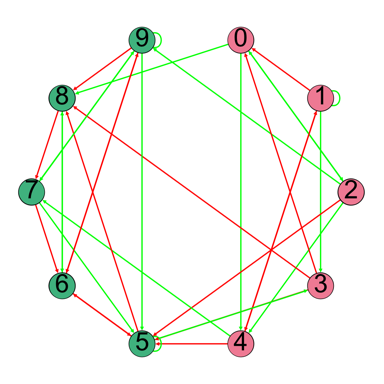
\includegraphics[width=\linewidth]{before-removing.png}
		\caption{Before removal}
	\end{subfigure}
	\begin{subfigure}[b]{0.45\linewidth}
		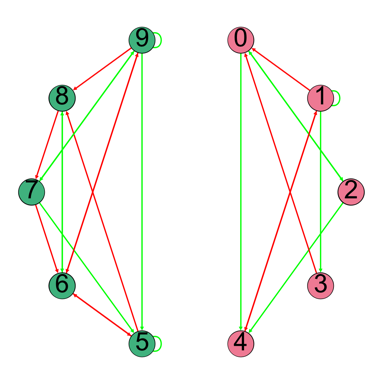
\includegraphics[width=\linewidth]{after-removing.png}
		\caption{After removal}
	\end{subfigure}
	\caption{Demonstration of inter-module connection removal}
	\label{fig:connection-removal}
\end{figure}
Originally, we suspected that this deviance was due to the fact that these modified solutions had a lower density than was expected from the evolutionary operations (sec 2.4), and thus may have been excluded from the search space. Nevertheless, further investigation revealed that the average number of edges for those networks that increased fitness values after triming their inter-module connections was approximately 30. That is, it was not due to the bias on the sparseness that caused this anomaly. 

In order to further comprehend this phenomenon on why our evolutionary simulations could not find a path to the trimed networks, we recorded the fitness value of removing one inter-module edge in turn, until deleting all of them. We plotted graphs as Figure \ref{fig:soto-path}, where x-axis represents the number of inter-module edges that have been discarded, y-axis represents the corresponding fitness values. Interestingly, most of our collected plots demonstrated a steady increasing trend for fitness vs deleting edge numbers, whereas genetic algorithms could not find these paths. 
\begin{figure}[h!]
	\centering
	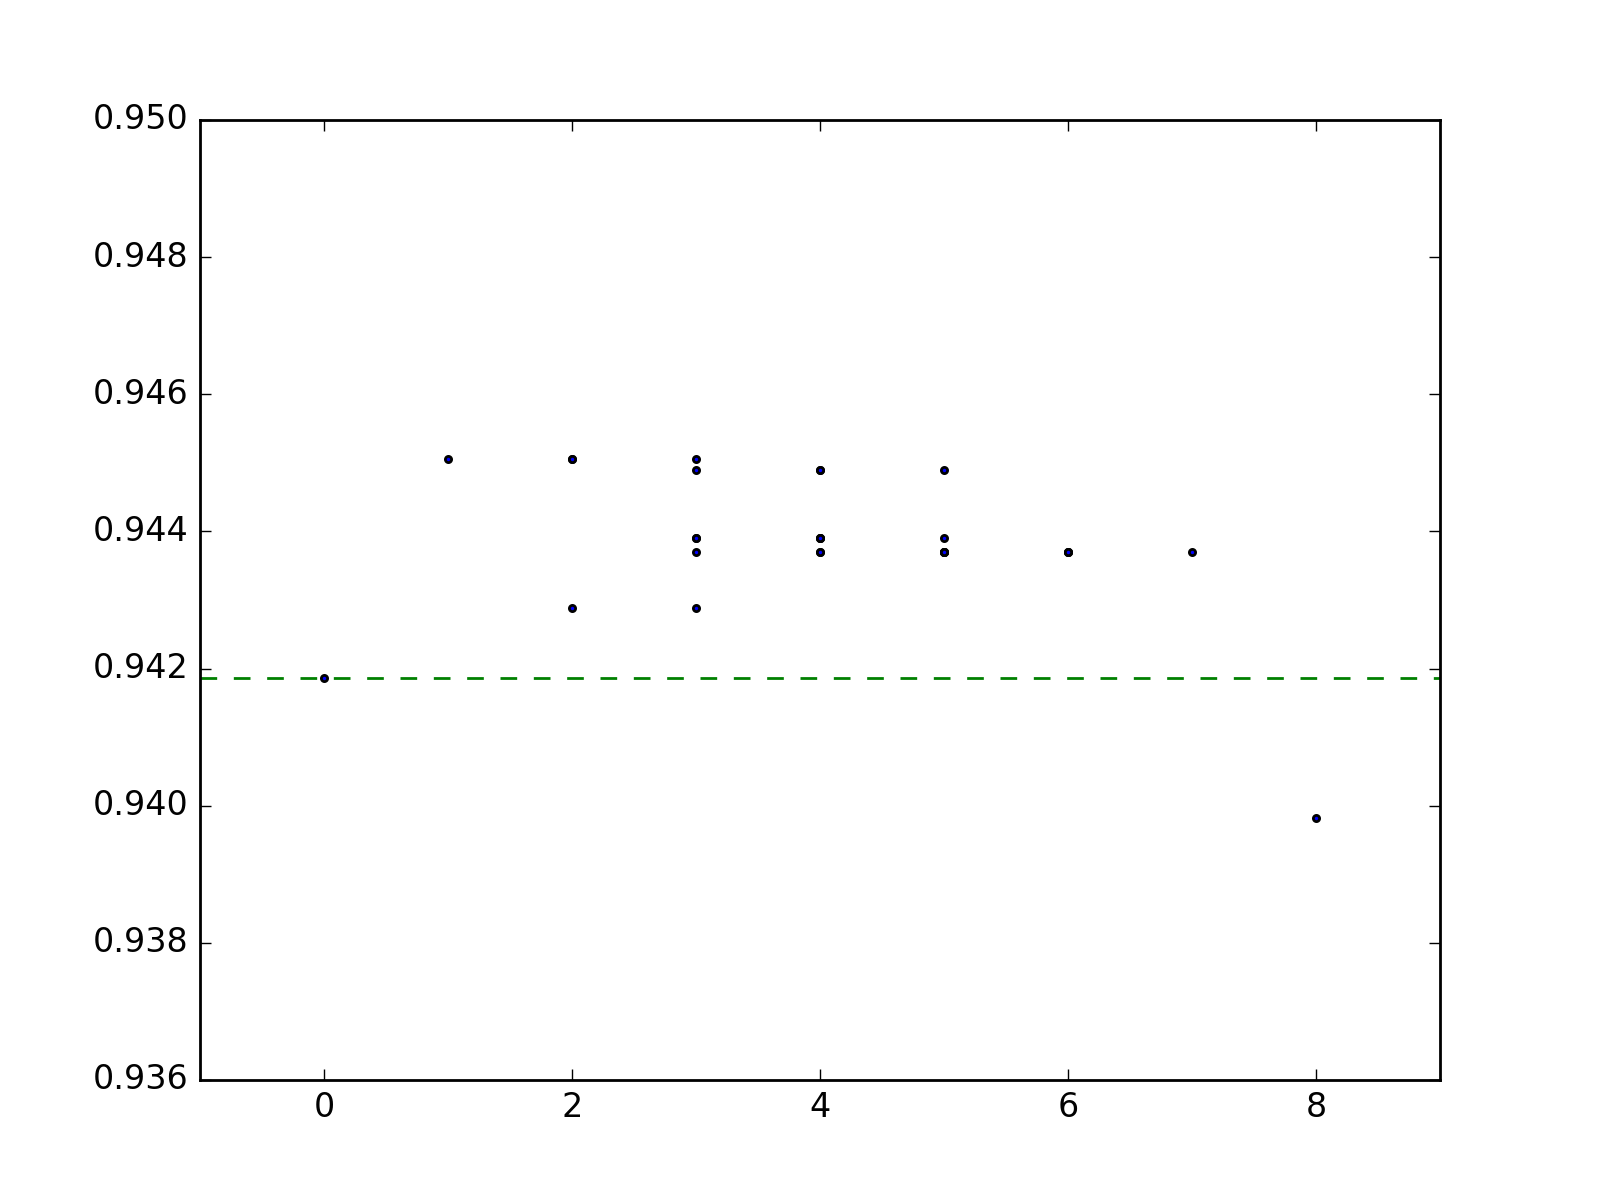
\includegraphics[width=\linewidth]{soto-path.png}
	\caption{A removing inter-module connection path}
	\label{fig:soto-path}
\end{figure}

\subsection{Fluctuant  landscapes are essential for generating modularity}
The stochastic fitness evaluation used by Espinosa-Soto and Wagner \cite{espinosa2010specialization} demonstrated much higher fitness and modularity Q score than Larson et al.'s deterministic fitness evaluation. Therefore, we hypothesized that a fluctuannt landscapes for individuals during the evolution might be necessary to develop high modularity. In order to verify this hypothesis, we collected the gene regulatory networks of the last generation, and mutated each network 9 times to generate their mutated neighbors. That is, each network would have 10 neighors, given including itself. Afterwards, we measured the fitness values of these neighors with the original target perturbations in the evolution and picked up thier maximum. In this fashion, we would have 40 maximum fitness values for both stochastic and deterministic fitness evaluation. Additionally, we also did the same process for the modularity Q score. Formally, a maximum value for a network $N$ is collected with the formula 
\begin{equation}
max(function(mutatedNeighbors(N)))
\end{equation}
where $function$ can either be $fitness$ or $modularity$. Subsequently, our statistical test indicated that fitness of stochastic neighbors did not demonstrate advantages, whereas their modularity Q scores were much higher than deterministic neighbors, as Tables \ref{table:4.12} and \ref{table:4.13} indicate. In general, in order to evolve out high modularity, a combination of gene specialization and a constantly changing environments will be desirable, instead of applying gene specialization alone. 
\begin{table}[h]
	\centering
	\caption{Results for comparsing stochastic and deterministic neighbor fitness}
	\label{table:4.12}
	\begin{tabular}{| p{0.3\linewidth}  | p{0.3\linewidth}  | p{0.3\linewidth} |} 
		\hline
		& Stochastic & Deterministic \\
		\hline
		Fitness & 0.9410 & 0.9323 \\ 
		\hline
		Q Score & 0.3374 & 0.1851 \\
		\hline
	\end{tabular}
\end{table}
\begin{table}[h]
	\centering
	\caption{Statistical significant results for comparsing stochastic and deterministic neighbor fitness}
	\label{table:4.13}
	\begin{tabular}{| p{0.5\linewidth}  | p{0.2\linewidth}  | p{0.2\linewidth}  |} 
		\hline
		& Fitness P & Q Score P \\
		\hline
		Deterministic < Stochastic & 0.7223 & 2.6879e-5 \\ 
		\hline
	\end{tabular}
\end{table}
Moreover, previously the statistics test revealed that the stochastic approach would lead to a higher fitness value, whereas this advantage disappeared when evaluating the fitness of mutated neighbors. Further investigation suggested that a deterministic, or static landscape may result in the searching getting stuck at the local optima. This is because for our 40 networks generated by deterministic fitness evaluation, the maximum fitness values for a network's neighbors were all from itself. That is, the neighbors of a network evolving in a static landscape always performed worse than themselves. Formally, for a network $N$, 
\begin{equation}
max(fitness(mutatedNeighbors(N))) = fitness(N)
\end{equation}
Furthermore, there existed a lot of networks produced by deterministic fitness evaluation whose fitness values were much lower (apprximately 0.88), compared to the rest of networks as well as those generated by stochastic fitness evaluation (approximately 0.93). We hypothesized that these low-performing networks are the cause on why statistically, fitness values generated by deterministic evaluation were lower than stochastic evaluation. Additionally, there may exist some correlation between getting stuck at local optima and modularity evolution. 

\subsection{More modular networks require fewer connections}
As previous results suggested, interactions between modules sometimes do not contribute to and even hamper the regulation activity of networks. That is, a network can gain a better performance by removing those inter-module connections, which indicates that modular networks require fewer connections in total. In order to justify this hypothesis, we collected both of the most and the least modular network among those fittest individuals from each evolutionary simulation in Section 4.1, using the dignonal crossover. That is, given two networks that have the same fitness value, we would like to discover whether the more modular one needs fewer connections. Our statistical test verified this hypothesis to be correct, as Table \ref{table:4.14} indicates. 
\begin{table}[h]
	\centering
	\caption{Results for verifying more modular networks require fewer connections}
	\label{table:4.14}
	\begin{tabular}{| p{0.225\linewidth}  | p{0.225\linewidth}  | p{0.225\linewidth} | p{0.225\linewidth} |} 
		\hline
		& Most Modular & Least Modular & Most < Least Modular p\\
		\hline
		Edge Number & 24.6 & 29.925 & 6.1913e-7\\ 
		\hline
	\end{tabular}
\end{table}

Clune et al. stated that the evolutionary origin of modularity is due to the cost associated with every connection in the network \cite{clune2013evolutionary}. They demonstrated this by their experiments indicating that there was a significant emergence of modular networks after imposing a penalty on the number of edges in the network \cite{clune2013evolutionary}.That is, modularity arose in order to minimise the connection costs. Specifically, they made simulated organisms evolve towards two objectives, namely to maximise the performance and to minimise the edge costs. However, in reality, biological organisms evolve in a single-objective fashion. That is, they are only selected under the pressure of fitting the living environments. Therefore, the theory stating that modularity comes from minimising connection costs may not be sufficiently plausible. 

Our results revealed a converse causality of Clune et al.'s explanation on modularity. To be specific, the connecting costs of modular networks are lower may be because modular networks need fewer edges to support their activities than non-modular ones. It may be also due to this, Clune et al. can recognise and select more modular systems by choosing structures in which there are fewer connections. Nevertheless, containing fewer edges is a property of more modular networks, not their evolutionary origin. 

